\documentclass[12pt,oneside]{article}
\usepackage{geometry}                                % See geometry.pdf to learn the layout options. There are lots.
\usepackage{listings}				% Permite utilizar lenguajes de programacion dentro de latex
\geometry{a4paper}                                           % ... or a4paper or a5paper or ... 
%\geometry{landscape}                                % Activate for for rotated page geometry
%\usepackage[parfill]{parskip}                    % Activate to begin paragraphs with an empty line rather than an indent
\usepackage{graphicx}                                % Use pdf, png, jpg, or epsß with pdflatex; use eps in DVI mode
                                                                % TeX will automatically convert eps --> pdf in pdflatex                
\usepackage{amssymb}

\usepackage[spanish]{babel}                        % Permite que partes automáticas del documento aparezcan en castellano.
\usepackage[utf8]{inputenc}                        % Permite escribir tildes y otros caracteres directamente en el .tex
\usepackage[T1]{fontenc}                                % Asegura que el documento resultante use caracteres de una fuente apropiada.

\usepackage{hyperref}                                % Permite poner urls y links dentro del documento
\usepackage{listings}

\title{Ejercicios de Programación - Sebesta}
\author{Lenguajes de Programación - ESPOL}

%\date{}                                                        % Activate to display a given date or no date

\begin{document}
\maketitle

	\section{Introducción}
	Las respuestas propuestas en este repositorio son producto del trabajo de los estudiantes de la materia ``Lenguajes de Programación'' de la ESPOL, correspondientes a las preguntas del libro de Robert Sebesta, Concepts of Programming Languages.

	\section{Preguntas y Respuestas}

		\subsection{Capítulo 5: Nombres, Enlaces y Alcances}
			\begin{itemize}
				\item {\bf Pregunta 4: Write a Python function that has subprograms nested three deep and in which each nested subprogram references variables defined in all of its enclosing subprogram}	
					\begin{center}
						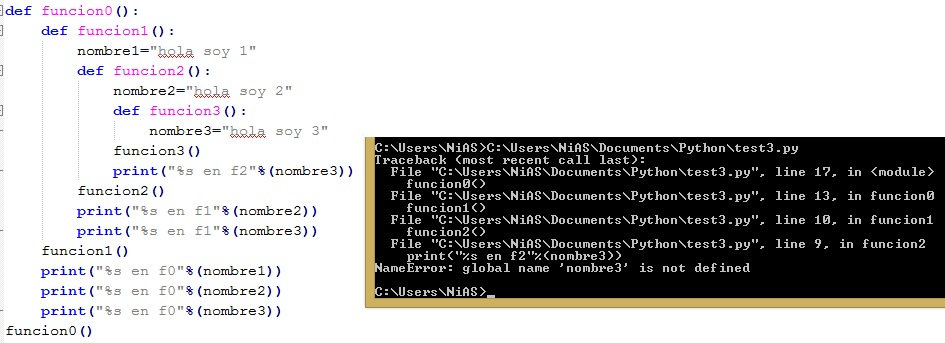
\includegraphics[scale=0.5]{Imagenes/6.jpg}\\
						NO EJECUTADO EN PYTHON: Variables no son declaradas globales
					\end{center}

				\item {\bf Pregunta 5: Write a C function that includes the following sequence of statements: x = 21;int x;x = 42; Run the program and explain the results. Rewrite the same code in C++ and Java and compare the results.}
					\begin{itemize}
						\item {Función en C}
							\begin{center}
							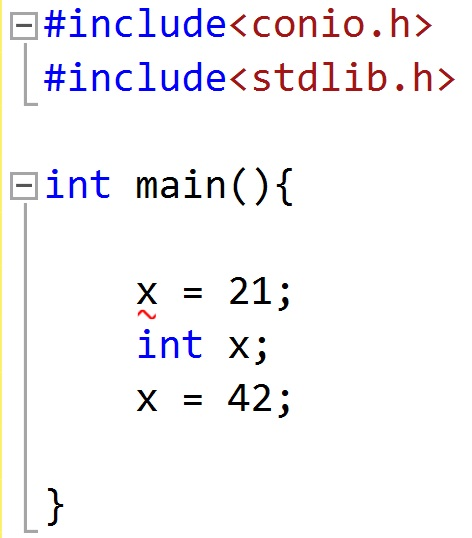
\includegraphics[scale=0.3]{Imagenes/1.jpg}\\
							NO COMPILA: error C2065: 'x' : identificador no declarado
							\end{center}
							ARGUMENTO: En el lenguaje C es necesario crear la variable o instanciarla de las siguientes formas antes de poder usarla o asignarle un valor: 
							\begin{itemize}
								\item{(tipo) (nombreVariable);}
									\\Ejemplo: int x;
								\item{(tipo) (nombreVariable)=(valor Inicial);}		
									\\Ejemplo: int x=10;							
							\end{itemize}

						\item {Función en C++}
							\\Sucede lo mismo que en C, el compilador de visual presenta los mismos errores, como si las tres lineas estuvieran mal escritas, aunque realmente es la primera.

						\item {Función en Java}
							\begin{center}
							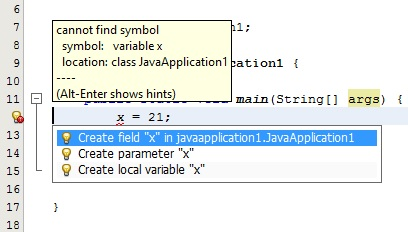
\includegraphics[scale=0.9]{Imagenes/2.jpg}\\
							NO COMPILA: error: cannot find symbol
							\end{center}		
							ARGUMENTO: En el lenguaje Java, el intérprete antes de compliar sugiere al programador crear la variable X como una variable de clase, y una vez compilado muestrar el error de que no puede encontrar el simbolo que se esta 									intentado usar, en este caso X.									
					\end{itemize}

				\item {\bf Pregunta 6: Write test programs in C++, Java, and C\# to determine the scope of a variable declared in a for statement. Specifically, the code must determine whether such a variable is visible after the body of the for statement.}
					\begin{itemize}
						\item {Función en C++}
							\begin{center}
								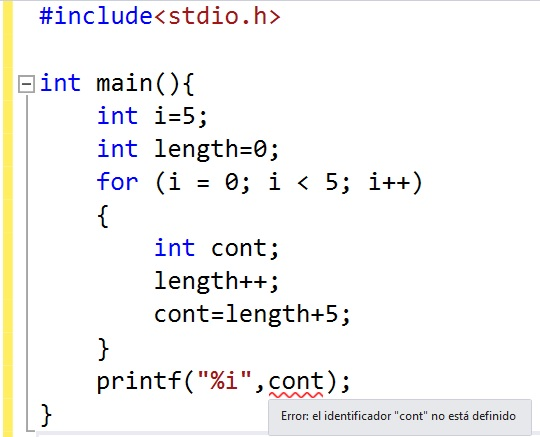
\includegraphics[scale=0.6]{Imagenes/3.jpg}\\
								NO COMPILA: No es visible despues de la sentencia for.
							\end{center}
						\item {Función en C\#}
							\begin{center}
								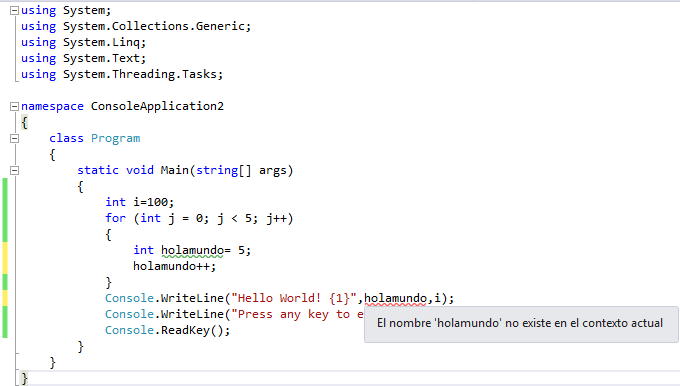
\includegraphics[scale=0.7]{Imagenes/4.jpg}\\
								NO COMPILA: No es visible despues de la sentencia for.
							\end{center}
							Es de notar que los avisos que muestra el intérprete son diferentes en los dos casos anteriores, en C++ nos dice que no existe definición de la variable que se quiere usar y por tanto no hay ningún valor que mostrar. En la 									siguiente, en C\# en cambio nos informa que no estamos en el mismo contexto y que por tanto la variable no es visible ni alcanzable.
					\end{itemize}
				\item {\bf Pregunta 7: Write three functions in C or C++: one that declares a large array statically, one that declares the same large array on the stack, and one that creates the same large array from the heap. Call each of the subprograms a large 					number of times (at least 100,000) and output the time required by each. Explain the results.}	
					\begin{center}
						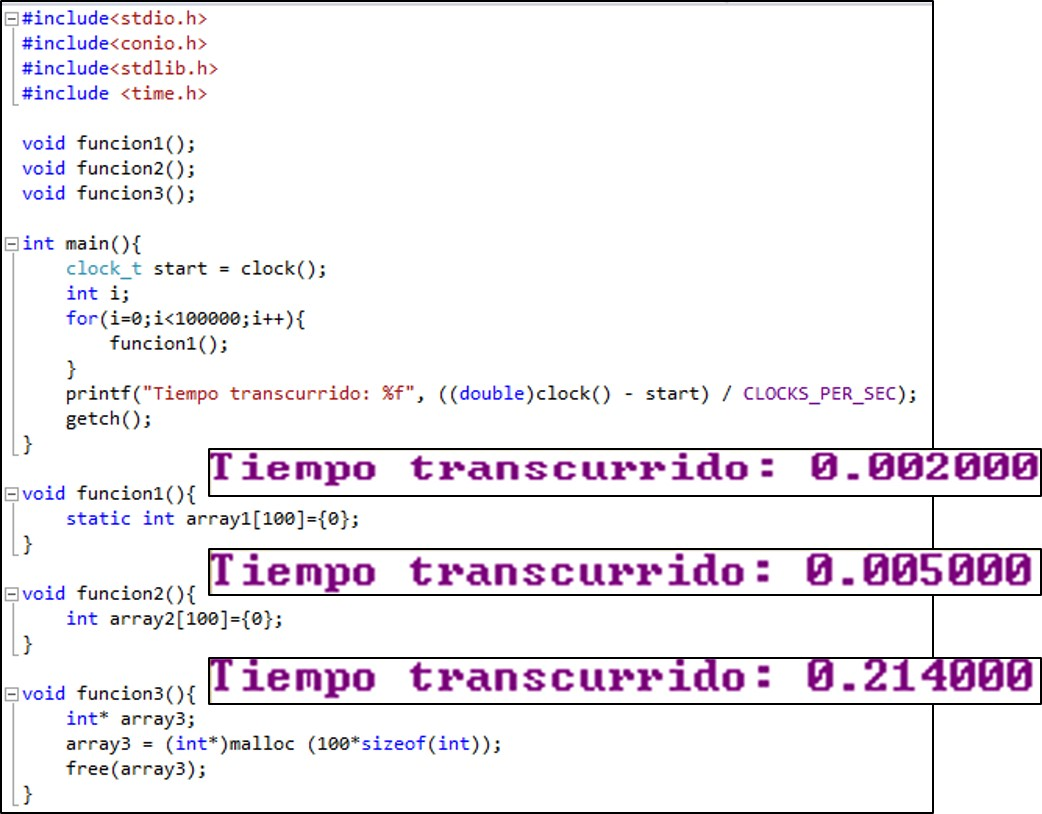
\includegraphics[scale=0.6]{Imagenes/5.jpg}\\
						EN C: Diferentes tiempos para diferentes funciones
					\end{center}
					ARGUMENTO: Las variables y vectores en C ocupan un tamaño fijo, el cuál es establecido antes de ejecutar el programa, por tanto no pueden variarlo durante esta ejecución. Por medio de punteros se puede reservar o liberar memoria 							dinámicamente, es decir, según se necesite. La Función malloc sirve para solicitar un bloque de memoria del tamaño suministrado como parámetro.
					Es notable que la petición MALLOC al querer reservar memoria toma más tiempo en su ejecución, pero también es importante entender que es una forma segura de programar, ya que estaremos seguros de que obtendremos la memoria que 							necesitemos para las variablemos que usemos, sin tener errores de memoria en tiempo de ejecución.
					Así que aunque en la imagén veamos que toma más tiempo ejecutar MALLOC es preferible su uso, para no arriesgarnos a errores de memoria.
		\end{itemize}


		\subsection{Capítulo 6: Tipos de Datos}
			\begin{itemize}
				\item {\bf Pregunta 1:Design a set of simple test programs to determine the type compatibility
rules of a C compiler to which you have access. Write a report of your findings.}

La estructura jerárquica de un programa normalmente se expresa utilizando reglas recursivas. Por ejemplo, se pueden dar las siguientes reglas como parte de la definición de expresiones:

    Cualquier identificador es una expresión.
    Cualquier número es una expresión.
    Si expresión1 y expresión2 son expresiones, entonces también lo son:
        expresión1 + expresión2
        expresión1 * expresión2
        ( expresión1 )

Las reglas 1 y 2 son reglas básicas (no recursivas), en tanto que la regla 3 define expresiones en función de operadores aplicados a otras expresiones.

La división entre análisis léxico y análisis sintáctico es algo arbitraria. Un factor para determinar la división es si una construcción del lenguaje fuente es inherentemente recursiva o no. Las construcciones léxicas no requieren recursión, mientras que las construcciones sintácticas suelen requerirla. No se requiere recursión para reconocer los identificadores, que suelen ser cadenas de letras y dígitos que comienzan con una letra. Normalmente, se reconocen los identificadores por el simple examen del flujo de entrada, esperando hasta encontrar un carácter que no sea ni letra ni dígito, y agrupando después todas las letras y dígitos encontrados hasta ese punto en un componente léxico llamado identificador.


\begin{lstlisting}[frame = single] 

int min(int a, int b) { 
  if (a < b) return a;
  return b;
}

	

int min(string a, string b) { 
  if (strcmp(a, b) < 0) return a;
  return b;
}


double x,y;
int a,b;
char c[ ],d[ ];

u = min(x,y);
v = min(a,b); 
w = min(c,d);
t = min(x,c); 

\end{lstlisting}
Error al tratar de comparar un tipo de
 dato double con un char[ ]

					
				\item {\bf Pregunta 2:Determine whether some C compiler to which you have access implements
the free function}
Memoria Dinámica 
Es memoria que se reserva en tiempo de ejecución. Su principal ventaja frente a la estática, es que su tamaño puede variar durante la ejecución del programa. (En C, el programador es encargado de liberar esta memoria cuando no la utilice más). El uso de memoria dinámica es necesario cuando a priori no conocemos el número de datos/elementos a tratar.

Memoria Estátiica
Es el espacio en memoria que se crea al declarar variables de cualquier tipo de dato (primitivas [int,char...] o derivados [struct,matrices,punteros...]). La memoria que estas variables ocupan no puede cambiarse durante la ejecución y tampoco puede ser liberada manualmente.

La función free sirve para liberar memoria que se asignó dinámicamente. Si el puntero es nulo, free no hace nada.


					
				\item {\bf Pregunta 7:Write a C program that does a large number of references to elements
of two-dimensioned arrays, using only subscripting. Write a second
program that does the same operations but uses pointers and pointer
arithmetic for the storage-mapping function to do the array references.
Compare the time efficiency of the two programs. Which of the two
programs is likely to be more reliable? Why?}

Programa 1
							\begin{lstlisting}[frame = single] 
#include <stdio.h>

#include <conio.h>

#include <string.h>

void main (void)

{

char cadena[10][70];
	for (i = 0; i <= 9; i++) {
		for (j = 0; j<=69; j++) {
		     printf("El valor es :%d",cadena[i][j] );

		}						
	}
}
							\end{lstlisting}
Accedimos a los elementos de la matriz por medio de subindice 

							Programa 2
							\begin{lstlisting}[frame = single] 


#define FILAS 10
#define COLS 70

int **matriz;
matriz = (int **)malloc (FILAS*sizeof(int *)*COLS);
 
for (i = 0; i <= FILAS; i++) {
		for (j = 0; j<=COLS; j++) {
		     printf("El valor es :%d",matriz** );

		}						
	}
matriz[i] = (int *) malloc (COLS*sizeof(int));

							\end{lstlisting}


Accedimos a cada elemento de la matriz por medio de punteros 
Lo mismo que en el caso de matrices unidimensionales, existen dos formas para acceder los elementos de matrices multidimensionales: mediante subíndices y mediante punteros. En cuanto a la primera, la forma de designar un elemento es: a[f][c], el primer subíndice indica la fila y el segundo la columna.

En caso de una matriz bidimensional m[A][B], la posición Pa,b respecto del comienzo del elemento m[a][b] viene determinado por: Pa,b = ( a * B ) + b. Es decir: (fila x total de columnas) + columna







						
\end{itemize}

		\subsection{Capítulo 7: Expresiones e Instrucciones de asignación}	
			\begin{itemize}
				\item {\bf Pregunta 1: Run the code given in Problem 13 (in the Problem Set) on some system that supports C to determine the values of sum1 and sum2. Explain the results.}
					\\El codigo:
					\lstset{language=C,basicstyle=\small\sffamily,numbers=left,numberstyle=\tiny,frame=tb,columns=fullflexible,showstringspaces=false}
					\begin{lstlisting}[frame=single]  % Start your code-block

int fun(int *k) {
	*k += 4;
	return 3 * (*k) - 1;
}

void main() {
	int i = 10, j = 10, sum1, sum2;
	sum1 = (i / 2) + fun(&i);
	sum2 = fun(&j) + (j / 2);
}
					\end{lstlisting}
					Nos devuelve sum1 = 46 y sum2 = 48
\begin{lstlisting}[frame=single]
sum1 = (i/2) + fun(&i) = 5 + 41 = 46  
//fun se calcula despues de obtener el valor de i/2
sum2 = fun(&j) + (j/2) = 41 + 7 = 48  
//fun se calcula antes de obtener el valor de j/2
\end{lstlisting}
					
				\item {\bf Pregunta 2: Rewrite the program of Programming Exercise 1 in C++, Java, and C\#, run them, and compare the results}
					\begin{itemize}
						\item {Programa en C++, C\#}
							\begin{lstlisting}[frame = single] 
class Program
    {
        static void Main(string[] args)
        {
            Program p = new Program();
            int i = 10,j=10,sum1,sum2;
            sum1 = (i / 2) + p.fun(ref i);
            sum2 = p.fun(ref j) + (j / 2);
            System.Console.WriteLine("sum1 = "+sum1);
            System.Console.WriteLine("sum2 = " + sum2);
            Console.Read();
        }
        public int fun(ref int k)
        {
            k = 4 + k;
            return 3*(k) - 1;
        }
    }

							\end{lstlisting}
							El programa retorna el mismo resultado que C
						\item {Programa en Java}
\lstset{language = java} 
\begin{lstlisting}[frame=single]
public class TestLP {
    public static void main(String[] args) {
        TestLP test = new TestLP();
        int i = 10, j = 10, sum1, sum2;
        sum1 = (i / 2) + test.fun(i);
        sum2 = test.fun(j) + (j / 2);
        System.out.println("sum1= " + sum1);
        System.out.println("sum2= " + sum2);
    }    
     public int fun(int k) {
        k += 4;
        return 3 * (k) - 1;
    }
}
\end{lstlisting}
							El programa retorna: sum1= 46 y sum2= 46, ya que no se pueden utilizar punteros en Java.
					\end{itemize}
				\item {\bf Pregunta 3: Write a test program in your favorite language that determines and outputs the precedence and associativity of its arithmetic and Boolean operators.}
\begin{lstlisting}[frame=single]
public class TestLP { 
     public static void main(String[] args) {
        boolean a;
        double e;
        a = true || false && false || false;
        System.out.println(a);
        a =false ||  true && false || false && false;
        System.out.println(a);
        e = 1 + 2 + 3 * 3 / 6.0;
        System.out.println(e);
        e = (1 + 2) + ((3 * 3) / 6.0);   
        System.out.println(e);
    }
}
\end{lstlisting}
					Como resultado obtenemos lo siguiente por consola
\begin{lstlisting}[frame=single]
true
false
4.5
4.5
\end{lstlisting}
					Lo que nos indica que en las operaciones booleanas el operador AND (\&\&) tiene mayor precedencia que el operador OR (||). En las operaciones aritmeticas el operador * tiene mayor precedencia que / y + 
										
				\item {\bf Pregunta 4: Write a Java program that exposes Java’s rule for operand evaluation order when one of the operands is a method call.}
\begin{lstlisting}[frame=single]
public class TestLP {
    public static void main(String[] args) {
        TestLP test = new TestLP();
        int a = 0, c;
        c = (a) + test.func(--a);
        System.out.println("c = " + c);
        System.out.println("a = " + a);
        a = 0;
        c = test.func(--a) + (a);
        System.out.println("c = " + c);
        System.out.println("a = " + a);
    }
    public int func(int c) {
        return c + 10;
    }
}
\end{lstlisting}
					El programa retorna:
\begin{lstlisting}[frame=single]
c = 9
a = -1
c = 8
a = -1
\end{lstlisting}
					Lo que nos muestra que las funciones se evaluan de izquierda a derecha
				\item {\bf Pregunta 5: Repeat Programming Exercise 5 with C++.}
					\lstset{language =[Sharp] C} 
					\begin{lstlisting}[frame=single]
class Program
    {
        static void Main(string[] args)
        {
            Program p = new Program();
            int a = 0, c;
            c = (a) + p.func(--a);
            System.Console.WriteLine("c = " + c);
            System.Console.WriteLine("a = " + a);
            a = 0;
            c = p.func(--a) + (a);
            System.Console.WriteLine("c = " + c);
            System.Console.WriteLine("a = " + a);
            Console.Read();
        }
        public int func(int c)
        {
            return c + 10;
        }
    }
					\end{lstlisting}
					El programa retorna:	
						\begin{center}
							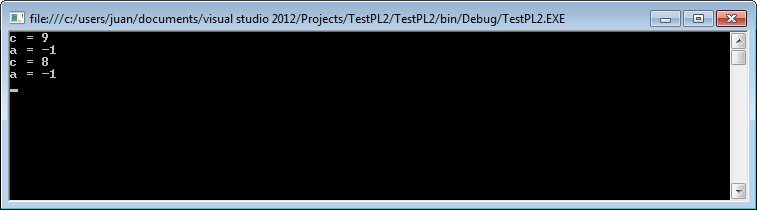
\includegraphics[scale=0.8]{Imagenes/c7-02}								
						\end{center}

				\item {\bf Pregunta 6: Repeat Programming Exercise 6 with C\#.}

					\lstset{language =[Sharp] C} 
					\begin{lstlisting}[frame=single]
class Program
    {
        static void Main(string[] args)
        {
            Program p = new Program();
            int a = 0, c;
            c = (a) + p.func(--a);
            System.Console.WriteLine("c = " + c);
            System.Console.WriteLine("a = " + a);
            a = 0;
            c = p.func(--a) + (a);
            System.Console.WriteLine("c = " + c);
            System.Console.WriteLine("a = " + a);
            Console.Read();
        }
        public int func(int c)
        {
            return c + 10;
        }
    }
					\end{lstlisting}
					El programa retorna:	
						\begin{center}
							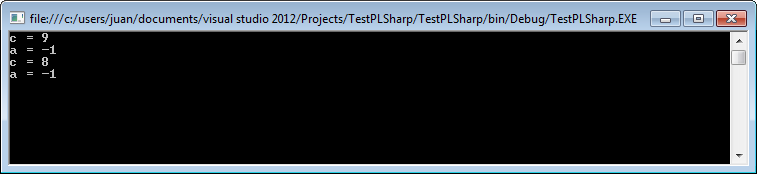
\includegraphics[scale=0.8]{Imagenes/c7-03}								
						\end{center}

				\item {\bf Pregunta 9: Write a program in either Java, C++, or C\# that performs a large number of floating-point operations and an equal number of integer operations and compare the time required.}
\lstset{language = java} 
\begin{lstlisting}[frame=single]
public class TestLP {
    public static void main(String[] args) {        
        int ae[] = new int[500000];
        float af[] = new float[500000];
        float  accf = 0;
        long t1, t2, t3, te, tf;
        int acce = 0;
        Random r = new Random();
        for(int i=0; i< 500000; i++){
            af[i]=r.nextFloat();
            ae[i]=r.nextInt(40);            
        }        
        t1= System.nanoTime();
        for(int e:ae){
            acce+=e;
        }
        t2=System.nanoTime();
        for(float f:af){
            accf+=f;
        }
        t3=System.nanoTime();
        te=t2-t1;
        tf=t3-t2;
        System.out.println("Total Entero = " + acce);
        System.out.println("Total Flotante = " + accf);
        System.out.println("Tiempo Entero = " + te);
        System.out.println("Tiempo Flotante = " + tf);
        System.out.println(t1);
        System.out.println(t2);
        System.out.println(t3);
    }    
}
\end{lstlisting}
					El tiempo Entero es de alrededor de 7 milisegundos, mientras que el tiempo de flotantes es de alrededor de 0.5 milisegundos
				\end{itemize}


		\subsection{Capítulo 8: Estructuras de Control}	
			\begin{itemize}
				\item {\bf Pregunta 3: Rewrite the following code segment using a multiple-selection statement
in the following languages:\\
if ((k == 1) || (k == 2)) j = 2 * k - 1\\
if ((k == 3) || (k == 5)) j = 3 * k + 1\\
if (k == 4) j = 4 * k - 1\\
if ((k == 6) || (k == 7) || (k == 8)) j = k - 2\\
a. Fortran 95 (you’ll probably need to look this one up)\\
b. Ada\\
c. C, C++, Java, or C\\
d. Python\\
e. Ruby\\
Assume all variables are integer type. Discuss the relative merits of the
use of these languages for this particular code.}	

Fortran  95
\begin{lstlisting}[frame=single]
if if ((k == 1) or (k == 2)) then 
 j = 2 * k - 1
elseif ((k == 3) or (k == 5)) then 
j = 3 * k + 1
elseif (k == 4) 
then j = 4 * k - 1
elseif ((k == 6) or (k == 7) or (k == 8))
then  j = k - 2
 end if 
\end{lstlisting}

C,C++,Java,or C
\begin{lstlisting}[frame=single]
if  ((k == 1) || (k == 2)) 
 j = 2 * k - 1
elseif ((k == 3) || (k == 5)) 
j = 3 * k + 1
elseif (k == 4) 
j = 4 * k - 1
elseif ((k == 6) || (k == 7) || (k == 8))
 j = k - 2 
\end{lstlisting}

Python 
\begin{lstlisting}[frame=single]
if  ((k == 1) or (k == 2)) :
 j = 2 * k - 1
elseif ((k == 3) or (k == 5)): 
j = 3 * k + 1
elseif (k == 4) :
j = 4 * k - 1
elseif ((k == 6) or (k == 7) or (k == 8)):
 j = k - 2 
\end{lstlisting}

Ruby
\begin{lstlisting}[frame=single]
if  ((k == 1) || (k == 2)) 
 j = 2 * k - 1
elseif ((k == 3) || (k == 5)) 
j = 3 * k + 1
elseif (k == 4) 
j = 4 * k - 1
elseif ((k == 6) || (k == 7) || (k == 8))
 j = k - 2 
end 
\end{lstlisting}


	
					
				\item {\bf Pregunta 4:Consider the following C program segment. Rewrite it using no gotos or breaks.\\
j = -3;\\
for (i = 0; i < 3; i++) {\\
	switch (j + 2) {\\
		case 3:\\
		case 2: j--; break;\\
		case 0: j += 2; break;\\
		default: j = 0;\\
	}\\
	if (j > 0) break;\\
	     j = 3 - i\\
}\\
}
\begin{lstlisting}[frame=single]
j = -3;
for (i = 0; i < 3; i++) {
		if (j + 2) == 3 

		elseif (j + 2) ==2 {
			j--;
			return ;
		}
		elseif (j + 2) == 0{
			 j += 2;
			 return;
		}
		else 
			 j = 0;
	}
	if ((j + 2) > 0)
	 return;
	 j = 3 - i
}

\end{lstlisting}



				\item {\bf Pregunta 5:In a letter to the editor of CACM, Rubin (1987) uses the following code
segment as evidence that the readability of some code with gotos is better
than the equivalent code without gotos. This code finds the first row
of an n by n integer matrix named x that has nothing but zero values.\\
for (i = 1; i <= n; i++) {\\
for (j = 1; j <= n; j++)\\
if (x[i][j] != 0)\\
goto reject;\\
println ('First all-zero row is:', i);\\
break;\\
reject:\\
}\\

Rewrite this code without gotos in one of the following languages: C,
C++, Java, C, or Ada. Compare the readability of your code to that of
the example code.}

\begin{lstlisting}[frame=single]
for (i = 1; i <= n; i++) {
	for (j = 1; j <= n; j++){
		if (x[i][j] != 0)
			continue;
	}
System.out.Println('First all-zero row is:'+ i);
break;

}
\end{lstlisting}

					
			\end{itemize}

		\subsection{Capítulo 9: SubProgramas}      
			\begin{itemize}
				\item {\bf Pregunta 1: Write a program in a language that you know to determine the ratio of the time required to pass a large array by reference and the time required to pass the same array by value. Make the array as large as possible on the 						machine and implementation you use. Pass the array as many times as necessary to get reasonably accurate timings of the passing operations.}
					\begin{center}
						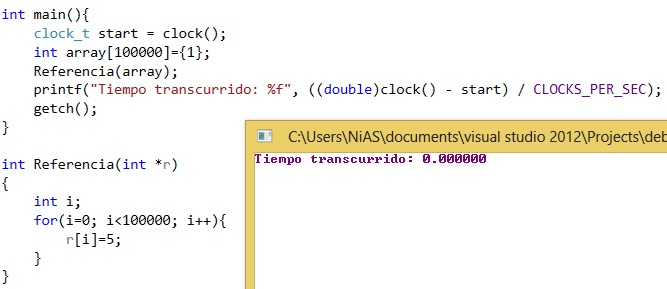
\includegraphics[scale=0.5]{Imagenes/7.jpg}\\
						POR REFERENCIA: Es notable que es más eficiente la ejecución al pasar un arreglo por referencia.\\
						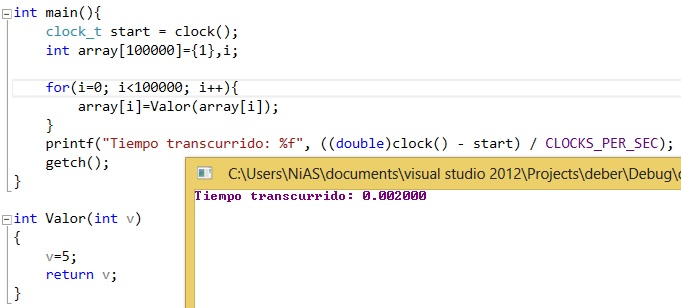
\includegraphics[scale=0.5]{Imagenes/8.jpg}\\
						POR VALOR: Se modificó la función para que hiciera lo mismo que la anterior, y notamos un cambio en los tiempos pero pasando cada elemento del arreglo por valor.
					\end{center}
					
			\end{itemize}


% Continuar con los siguientes capítulos y ejercicios:
% Ch6: 1, 2, 7
% Ch7: 1 - 6, 9
% Ch8: 3, 4, 5
% Ch9: 1, 5
% Recuerden que todos corresponden a las secciones de "Programming Exercises".

\end{document}
